\documentclass[11pt,a4paper]{article}

\usepackage[margin=2.4cm]{geometry}
\usepackage[utf8]{inputenc}
\usepackage{lmodern}
\usepackage[T1]{fontenc}
\usepackage{amsmath,amssymb,amsfonts,amsthm}
\usepackage{mathtools}
\usepackage{booktabs}
\usepackage{array}
\usepackage{enumitem}
\usepackage{graphicx}
\usepackage{listings}
\usepackage{xcolor}
\usepackage{hyperref}
\hypersetup{colorlinks=true, linkcolor=blue, citecolor=blue, urlcolor=blue}

\lstset{
  language=Python,
  basicstyle=\ttfamily\footnotesize,
  keywordstyle=\bfseries,
  commentstyle=\itshape\color{gray},
  breaklines=true,
  frame=single,
  columns=fullflexible,
  keepspaces=true,
  showstringspaces=false,
  aboveskip=0.6em,
  belowskip=0.6em,
}

\theoremstyle{definition}
\newtheorem{definition}{Definici\'on}
\newtheorem{remark}{Observaci\'on}

\newcommand{\vect}[1]{\boldsymbol{#1}}
\newcommand{\matr}[1]{\mathbf{#1}}
\newcommand{\R}{\mathbb{R}}
\DeclareMathOperator{\diag}{diag}
\DeclareMathOperator{\Cov}{Cov}

\title{Sustento te\'orico del CRB polar NLOS\\[4pt]
\large Matem\'atica de nuestra formulaci\'on e implementaci\'on}
\author{Obstacle Detection Study}
\date{\today}

\begin{document}
\maketitle

\begin{abstract}
Este documento es el \textbf{sustento te\'orico} del an\'alisis CRB que realizamos
en el repositorio (\texttt{simulation\_polar\_clean.ipynb},
\texttt{crb\_polar\_functions.py}).
La estructura es \emph{similar} a la del writeup de Active Corner Camera
(parametrizaci\'on polar, Poisson, Fisher, cotas $3\sigma$), pero \textbf{no es
una copia}: adoptamos un modelo de medida discreto (suma sobre tri\'angulos y
bins), estimamos $\vect{\psi}=[\rho,\varphi,h]^{\mathsf T}$ (Fisher $3\times 3$),
tratamos el ancho $w$ como fijo, y obtenemos derivadas por diferencias finitas.
El objetivo es poder citar este texto como respaldo matem\'atico de lo que el
c\'odigo calcula.
\end{abstract}

\tableofcontents
\bigskip\hrule\bigskip

%==============================================================================
\section{Objetivo del an\'alisis}
\label{sec:objetivo}
%==============================================================================

Queremos acotar cu\'an precisamente se puede localizar una faceta oculta en el
plano del suelo a partir de un histograma SPAD$\times$tiempo de fotones,
bajo el modelo de Poisson. La herramienta es la \textbf{cota de Cram\'er--Rao}
(CRB) asociada a la matriz de informaci\'on de Fisher de la medida esperada.

En nuestra formulaci\'on:
\begin{enumerate}[nosep]
    \item la escena se parametriza en polares $(\rho,\varphi)$;
    \item la medida esperada $g$ se obtiene de un simulador de transporte
          discreto (rebote faceta $\to$ FOV);
    \item el Jacobiano $\partial g/\partial\vect{\psi}$ se aproxima por
          diferencias finitas sobre \textbf{todos} los bins;
    \item reportamos $\sigma_\rho$, $\sigma_\varphi$, $\sigma_h$ y regiones
          $3\sigma$ marginales en $(\rho,\varphi)$.
\end{enumerate}

\begin{remark}[Relaci\'on con el writeup]
El writeup de Seidel et al.\ usa el mismo esp\'iritu (Fisher de Poisson +
oclusi\'on por arista) con $\vect{\Psi}=[\alpha,\rho,\varphi,h]$ y derivadas
anal\'iticas bajo el integrando.
Nosotros \textbf{heredamos la idea}, pero el objeto matem\'atico que
analizamos es el de nuestro forward discreto y
$\vect{\psi}=[\rho,\varphi,h]$ (sin albedo $\alpha$).
\end{remark}

\begin{remark}[Estado actual del c\'odigo]
La prueba can\'onica que reportamos \textbf{incluye la altura} $h$ como
par\'ametro desconocido (\texttt{estimate\_height=True}): Fisher $3\times 3$,
pasos FD $[\delta\rho,\delta\varphi,\delta h]$, y elipses $3\sigma$
\textbf{marginales} en $(\rho,\varphi)$ (la incertidumbre de $h$ ya est\'a
absorbida al invertir $\matr{I}$). El ancho $w$ permanece fijo.
\end{remark}

%==============================================================================
\section{Parametrizaci\'on de la escena}
\label{sec:param}
%==============================================================================

\subsection{Pose polar}
Una faceta vertical se coloca en el plano $z=0$ (base) con
\begin{equation}
    x = \rho\cos\varphi,
    \qquad
    y = \rho\sin\varphi,
    \qquad
    \rho>0,\quad \varphi\in(0,\pi)
    \label{eq:polar}
\end{equation}
en la convenci\'on del simulador ($X,Y$ = suelo, $Z$ = altura).
El vector de par\'ametros \textbf{estimados} en el CRB es, por defecto,
\begin{equation}
    \vect{\psi}
    =
    \begin{bmatrix}\rho\\ \varphi\\ h\end{bmatrix},
    \label{eq:psi}
\end{equation}
donde $h$ es la altura vertical de la faceta.
La Fisher resultante es $3\times 3$ y reportamos
$\sigma_\rho$, $\sigma_\varphi$ y $\sigma_h$.
Las elipses en el plano $(\rho,\varphi)$ usan el bloque $2\times 2$
\textbf{marginal} de $\matr{I}^{+}$ (altura desconocida).

La normal media de la faceta se orienta hacia la arista,
$\hat{\vect{n}}\approx[-\cos\varphi,-\sin\varphi,0]$, para que mire al
lado visible/l\'aser.

\subsection{Ancho fijo; altura estimada}
El ancho horizontal $w$ permanece como par\'ametro de escena fijo
(no se diferencia). La altura $h$ s\'i entra en $\vect{\psi}$ y se acota
con $\sigma_h=\sqrt{[\matr{I}^{+}]_{22}}$.
En el mesh (antes del pitch $\approx\pi/2$)
\begin{equation}
    \mathrm{scale}_x = \frac{w}{\mathrm{extent}_X},
    \qquad
    \mathrm{scale}_y = \frac{h}{\mathrm{extent}_Y},
\end{equation}
de modo que $h$ es independiente de $w$.
Por defecto $h_0=1\,\mathrm{m}$.

Opcionalmente se puede fijar $h$ (\texttt{estimate\_height=False}) y
recuperar el CRB $2\times 2$ solo en $(\rho,\varphi)$.

%==============================================================================
\section{Modelo de medida discreto}
\label{sec:medida}
%==============================================================================

\subsection{Cubo transitorio y tasa de Poisson}
Sea $y(\vect{\psi})\in\R^{H\times W\times T}$ el histograma esperado de
fotones (sin ruido de muestreo) producido por el forward.
Con fondo (dark counts / ambient) $b\ge 0$,
\begin{equation}
    g(\vect{\psi})
    =
    y(\vect{\psi}) + b,
    \qquad
    \vect{g}
    =
    \operatorname{vec}\bigl(g(\vect{\psi})\bigr)\in\R^{N},
    \quad
    N = HWT.
    \label{eq:g}
\end{equation}
Cada bin $q=1,\ldots,N$ se modela como
\begin{equation}
    X_q \;\sim\; \mathrm{Poisson}\bigl(g_q(\vect{\psi})\bigr)
    \quad\text{independientes}.
    \label{eq:poisson}
\end{equation}

\subsection{Construcci\'on de $y$: suma como integral}
El writeup escribe $y_q$ como integral de una radiancia $L_h$ sobre el
p\'ixel y el bin temporal.
Nosotros \textbf{definimos} $y$ mediante una cuadratura asociada al mesh:

\begin{enumerate}[leftmargin=1.4cm]
    \item Descomponer la faceta (y opcionalmente paredes) en tri\'angulos de
          centro $\vect{c}$, \'area $A$ y normal $\hat{\vect{n}}$.
    \item Para cada muestra espacial $\vect{p}_f$ del FOV (centros de SPAD
          y subp\'ixeles), acumular
    \begin{equation}
        \Delta y
        \propto
        I_{\mathrm{laser}}\,
        A\,
        [\hat{\vect{n}}\cdot\hat{\vect{u}}_1]_+
        \cdots
        [\hat{\vect{n}}_f\cdot\hat{\vect{u}}_4]_+
        \,\frac{1}{4\pi^{2}\,d_1^{2}\,d_2^{2}},
        \label{eq:dy}
    \end{equation}
          con $d_1=\|\vect{p}_l-\vect{c}\|$, $d_2=\|\vect{p}_f-\vect{c}\|$.
    \item Asignar el retardo a un bin
    \begin{equation}
        j
        =
        \left\lceil
            \frac{d_1+d_2}{c\,\Delta t}
        \right\rceil
        \label{eq:bin}
    \end{equation}
          ($\Delta t=$\texttt{bin\_size}).
\end{enumerate}

En notaci\'on compacta,
\begin{equation}
    y_q
    =
    \sum_{\triangle}
    \sum_{\mathrm{sub}\,\in\,P_i}
    \mathbf{1}\{\mathrm{visible}\}
    \,\mathbf{1}\{j=q_t\}
    \,\Delta y_{\triangle,\mathrm{sub}}.
    \label{eq:y-sum}
\end{equation}
Esto \textbf{es} nuestra ``integral'' de medida: una suma de Riemann sobre
elementos de superficie y muestras espaciales, con pulso idealizado como masa
en un solo bin.

\subsection{Oclusi\'on / ``sombra'' (c\'omo se calcula)}
\label{sec:sombra}
La esquina oculta caminos faceta$\to$FOV que no cruzan la arista visible.
En el c\'odigo (\texttt{simulation}), para cada tri\'angulo de centro
$\vect{c}=(c_x,c_y,c_z)$ y cada muestra de c\'amara $\vect{p}_f=(p_x,p_y,p_z)$:

\begin{enumerate}[nosep]
    \item Se traza la recta en el plano $XY$ entre $\vect{c}$ y $\vect{p}_f$:
    \[
        m=\frac{c_y-p_y}{c_x-p_x},\qquad
        b=c_y-m\,c_x.
    \]
    \item Intersecci\'on con la arista $x=0$:
    \[
        \texttt{xint}=-b/m
    \]
    (NaN si el denominador o $m$ son nulos).
    \item M\'ascara de caminos \emph{no ocluidos}:
    \begin{equation}
        \texttt{noc}
        =
        \bigl(\texttt{xint}\ \text{finito}\bigr)
        \land
        (\texttt{xint}>0).
        \label{eq:noc}
    \end{equation}
    \item Solo los \'indices con \texttt{noc=True} reciben intensidad
          $\Delta y$ en el histograma. El resto queda en $y=0$
          (p\'ixel / bin en sombra para esa geometr\'ia).
\end{enumerate}

En la CRB \textbf{no descartamos} esos bins: $g=\mathrm{vec}(y+b)$ incluye
$y\approx 0$ en sombra. Al perturbar $\varphi$ o $h$ por FD, un bin puede
pasar de sombra a iluminado (o al rev\'es) y eso aparece en $\matr{J}$.
Eso es ``incluir los p\'ixeles sombreados en las derivadas''.

%==============================================================================
\section{Verosimilitud, score y Fisher}
\label{sec:fisher}
%==============================================================================

\subsection{Log-verosimilitud}
Con observaciones $x_q$ y tasa $g_q(\vect{\psi})$,
\begin{equation}
    \ell(\vect{\psi})
    =
    \sum_{q=1}^{N}
    \Bigl(
        x_q\log g_q(\vect{\psi})
        -
        g_q(\vect{\psi})
        -
        \log(x_q!)
    \Bigr).
    \label{eq:ll}
\end{equation}

\subsection{Score y matriz de informaci\'on}
Derivando respecto a $\psi_m$ y tomando esperanza bajo el modelo
(\ref{eq:poisson}),
\begin{equation}
    I_{mk}(\vect{\psi})
    =
    \sum_{q=1}^{N}
    \frac{1}{g_q(\vect{\psi})}
    \frac{\partial g_q}{\partial\psi_m}
    \frac{\partial g_q}{\partial\psi_k},
    \qquad
    m,k\in\{\rho,\varphi,h\}.
    \label{eq:I}
\end{equation}
En forma matricial, con Jacobiano $\matr{J}\in\R^{N\times 3}$ cuyas columnas
son $\partial\vect{g}/\partial\rho$, $\partial\vect{g}/\partial\varphi$ y
$\partial\vect{g}/\partial h$,
\begin{equation}
    \matr{I}
    =
    \matr{J}^{\mathsf T}
    \diag\bigl(1/\vect{g}\bigr)\,
    \matr{J}.
    \label{eq:I-mat}
\end{equation}
Esta es la misma estructura Fisher--Poisson del writeup; cambia el dominio
de par\'ametros ($3$ en lugar de $4$, sin albedo) y c\'omo se obtienen $g$ y $\matr{J}$.

\begin{remark}[Regularizaci\'on num\'erica]
Si $g_q=0$, el t\'ermino $1/g_q$ no est\'a definido.
En la implementaci\'on usamos $g_q\leftarrow\max(g_q,\varepsilon)$ con
$\varepsilon\ll 1$ (\texttt{fisher\_eps}).
\end{remark}

%==============================================================================
\section{Cota de Cram\'er--Rao y regiones de incertidumbre}
\label{sec:crb}
%==============================================================================

\subsection{CRB}
Para un estimador insesgado $\hat{\vect{\psi}}$ de $\vect{\psi}$,
\begin{equation}
    \Cov(\hat{\vect{\psi}})
    \;\succeq\;
    \matr{I}(\vect{\psi})^{-1},
\end{equation}
en el sentido de matrices semidefinidas positivas
(usamos la pseudoinversa $\matr{I}^{+}$ si $\matr{I}$ es mal condicionada).
Definimos
\begin{equation}
    \sigma_\rho
    =
    \sqrt{[\matr{I}^{+}]_{00}},
    \qquad
    \sigma_\varphi
    =
    \sqrt{[\matr{I}^{+}]_{11}},
    \qquad
    \sigma_h
    =
    \sqrt{[\matr{I}^{+}]_{22}},
    \qquad
    \sigma_{\mathrm{tang}}
    =
    \rho\,\sigma_\varphi.
\end{equation}
$\sigma_{\mathrm{tang}}$ convierte la incertidumbre angular en metros de arco
en la pose nominal.

\subsection{Elipse $3\sigma$ en $(\rho,\varphi)$}
Sea $\Sigma$ el bloque $2\times 2$ \textbf{marginal} de $\matr{I}^{+}$ en
$(\rho,\varphi)$ (altura desconocida ya absorbida al invertir la Fisher $3\times 3$).
Con autodescomposici\'on $\Sigma=U\diag(\lambda)U^{\mathsf T}$ y $k=3$,
\begin{equation}
    \begin{bmatrix}\rho(t)\\ \varphi(t)\end{bmatrix}
    =
    \begin{bmatrix}\rho_0\\ \varphi_0\end{bmatrix}
    +
    U\,\diag(k\sqrt{\lambda})\,
    \begin{bmatrix}\cos t\\ \sin t\end{bmatrix},
    \quad
    t\in[0,2\pi).
    \label{eq:ellipse-param}
\end{equation}
Esta curva es una elipse en el plano de par\'ametros $(\rho,\varphi)$.
Al dibujarla en ejes polares (radio $=\rho$, \'angulo $=\varphi$) se obtienen
las ``burbujas'' an\'alogas a las del writeup --- \textbf{sin} proyectar antes
a $(x,y)$.

Esa es la visualizaci\'on can\'onica de nuestro estudio
(\texttt{use\_physical\_region=False}).

\subsection{Pushforward opcional a metros en el suelo}
Si se desea interpretar la incertidumbre en coordenadas cartesianas,
\begin{equation}
    \matr{A}
    =
    \begin{bmatrix}
        \cos\varphi_0 & -\rho_0\sin\varphi_0 \\
        \sin\varphi_0 & \rho_0\cos\varphi_0
    \end{bmatrix},
    \qquad
    \Sigma_{xy}
    =
    \matr{A}\,\Sigma\,\matr{A}^{\mathsf T}.
\end{equation}
La elipse $3\sigma$ en $(x,y)$ es la regi\'on espacial linealizada.
Reparametrizar esa curva a polares para un plot polar la \textbf{deforma}
(apariencia de ``gota'') cuando $\sigma$ es grande: no es un error de Fisher,
es un efecto de visualizaci\'on.

%==============================================================================
\section{Derivadas: aproximaci\'on por diferencias finitas}
\label{sec:fd}
%==============================================================================

El forward $g(\vect{\psi})$ incluye m\'aximos, techos de bin y la m\'ascara
\texttt{noc}: no es diferenciable en todos los puntos.
Por ello no usamos derivadas anal\'iticas bajo un integrando continuo, sino
el Jacobiano num\'erico
\begin{equation}
    \frac{\partial\vect{g}}{\partial\psi_m}
    \;\approx\;
    \frac{
        \vect{g}(\vect{\psi}_0+\delta_m\vect{e}_m)
        -
        \vect{g}(\vect{\psi}_0-\delta_m\vect{e}_m)
    }{2\delta_m},
    \label{eq:central}
\end{equation}
$m\in\{\rho,\varphi,h\}$ (diferencias centrales, $\mathcal{O}(\delta^{2})$).

Opcionalmente, extrapolaci\'on de Richardson de orden $\mathcal{O}(\delta^{4})$
sobre el mismo forward.

\begin{remark}
Al perturbar $\varphi$ o $h$, p\'ixeles pueden pasar de iluminados a ocluidos
(o al rev\'es). El FD captura ese salto de frontera en $\matr{J}$: es el
an\'alogo num\'erico de diferenciar a trav\'es del Heaviside del writeup.
\end{remark}

Costo t\'ipico (central, $3$ par\'ametros): $7$ evaluaciones de $g$ por pose
(nominal + $2$ por par\'ametro).

%==============================================================================
\section{Fondo y oclusi\'on en la CRB}
\label{sec:fondo}
%==============================================================================

Como $I_{mk}$ pesa cada bin con $1/g_q$ y $g_q=y_q+b$, aumentar $b$ diluye la
informaci\'on y empeora la CRB.

La oclusi\'on se calcula en el forward (Sec.~\ref{sec:sombra}). En la CRB
usamos \textbf{todos} los bins: sombras entran como $y\approx 0$ y, al
diferenciar, como saltos de frontera en $\matr{J}$. No hay paso que descarte
p\'ixeles sombreados antes del Fisher.

%==============================================================================
\section{Cadena matem\'atica implementada}
\label{sec:cadena}
%==============================================================================

\begin{equation}
\begin{aligned}
    \vect{\psi}_0
    &\;\xrightarrow{\ \text{forward discreto}\ }\;
    y_0,\;\;
    \vect{g}_0=\operatorname{vec}(y_0+b) \\[4pt]
    &\;\xrightarrow{\ \text{FD central/Richardson}\ }\;
    \matr{J}
    \approx
    \frac{\partial\vect{g}}{\partial\vect{\psi}^{\mathsf T}}
    \Big|_{\vect{\psi}_0} \\[4pt]
    &\;\xrightarrow{\ \text{Fisher Poisson}\ }\;
    \matr{I}
    =
    \matr{J}^{\mathsf T}\diag(1/\vect{g}_0)\,\matr{J} \\[4pt]
    &\;\xrightarrow{\ \text{CRB}\ }\;
    \Sigma=\matr{I}^{+},\quad
    \text{elipse }3\sigma\text{ en }(\rho,\varphi).
\end{aligned}
\label{eq:pipeline}
\end{equation}

Esto es exactamente lo que orquesta \texttt{compute\_crb\_polar}
(y \texttt{compute\_crb\_grid\_polar} sobre una malla de poses).

%==============================================================================
\section{Qu\'e es igual y qu\'e no respecto al writeup}
\label{sec:vs-pdf}
%==============================================================================

\begin{center}
\small
\begin{tabular}{@{}p{3.2cm}p{5.5cm}p{5.5cm}@{}}
\toprule
 & Writeup (PDF) & Nuestra formulaci\'on \\
\midrule
Par\'ametros &
$[\alpha,\rho,\varphi,h]$ &
$[\rho,\varphi,h]$; $w$ fijo \\
Medida $y_q$ &
$\iint L_h\,d\vect{p}\,dt$ &
Suma (\ref{eq:y-sum}) sobre mesh + bins \\
Oclusi\'on &
Heaviside anal\'itico &
M\'ascara \texttt{noc}/\texttt{xint} \\
$\partial g/\partial\psi$ &
Derivada bajo el integrando &
Diferencias finitas \\
Fisher &
$\sum (\partial_m g)(\partial_k g)/g$ &
Id\'em, eq.~(\ref{eq:I})--(\ref{eq:I-mat}) \\
Regiones &
Burbujas $3\sigma$ en polar &
Elipse (\ref{eq:ellipse-param}) en $(\rho,\varphi)$ \\
\bottomrule
\end{tabular}
\end{center}

%==============================================================================
\section{Figuras de regiones CRB (con $h$ y sin $h$)}
\label{sec:figura}
%==============================================================================

Misma malla de poses
\[
\rho\in\{0{,}5,\,1{,}0,\,1{,}5\}\,\mathrm{m},
\qquad
\varphi\in\{30^\circ,60^\circ,90^\circ,120^\circ,150^\circ\},
\]
$w=0{,}5\,\mathrm{m}$, geometr\'ia $h=1{,}0\,\mathrm{m}$, fondo $b=0{,}1$,
FD central, elipses $3\sigma$ en $(\rho,\varphi)$
(\texttt{use\_physical\_region=False}).

Dos variantes (el t\'itulo del PNG indica qu\'e se estima):
\begin{itemize}[nosep]
    \item \textbf{CRB$(\rho,\varphi,h)$}
          (\texttt{plots/crb\_standard\_regions.png}):
          se estiman $\rho$, $\varphi$ y $h$; Fisher $3\times 3$;
          elipse marginal en $(\rho,\varphi)$.
    \item \textbf{CRB$(\rho,\varphi)$}
          (\texttt{plots/crb\_standard\_regions\_fixed\_h.png}):
          solo $\rho$ y $\varphi$; $h$ fija en la geometr\'ia;
          Fisher $2\times 2$.
\end{itemize}
En general las elipses de CRB$(\rho,\varphi,h)$ son m\'as grandes que las de
CRB$(\rho,\varphi)$ (peor cota: un par\'ametro extra desconocido).

\begin{figure}[ht]
\centering
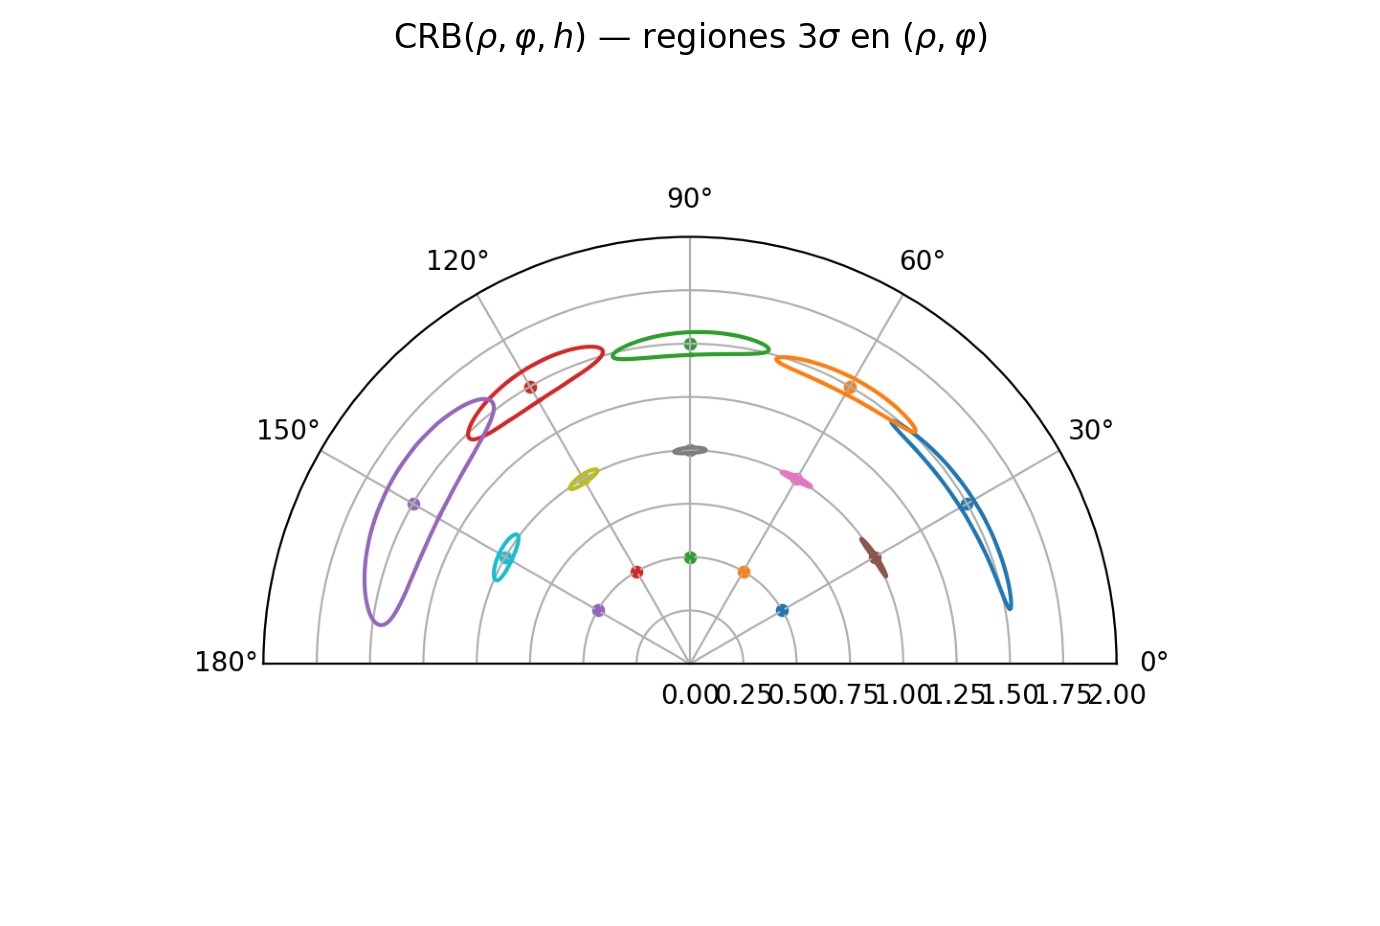
\includegraphics[width=0.92\textwidth]{../plots/crb_standard_regions.png}
\caption{CRB$(\rho,\varphi,h)$: regiones $3\sigma$ en $(\rho,\varphi)$. Archivo: \texttt{plots/crb\_standard\_regions.png}.}
\label{fig:crb-regions-h}
\end{figure}

\begin{figure}[ht]
\centering
\IfFileExists{../plots/crb_standard_regions_fixed_h.png}{%
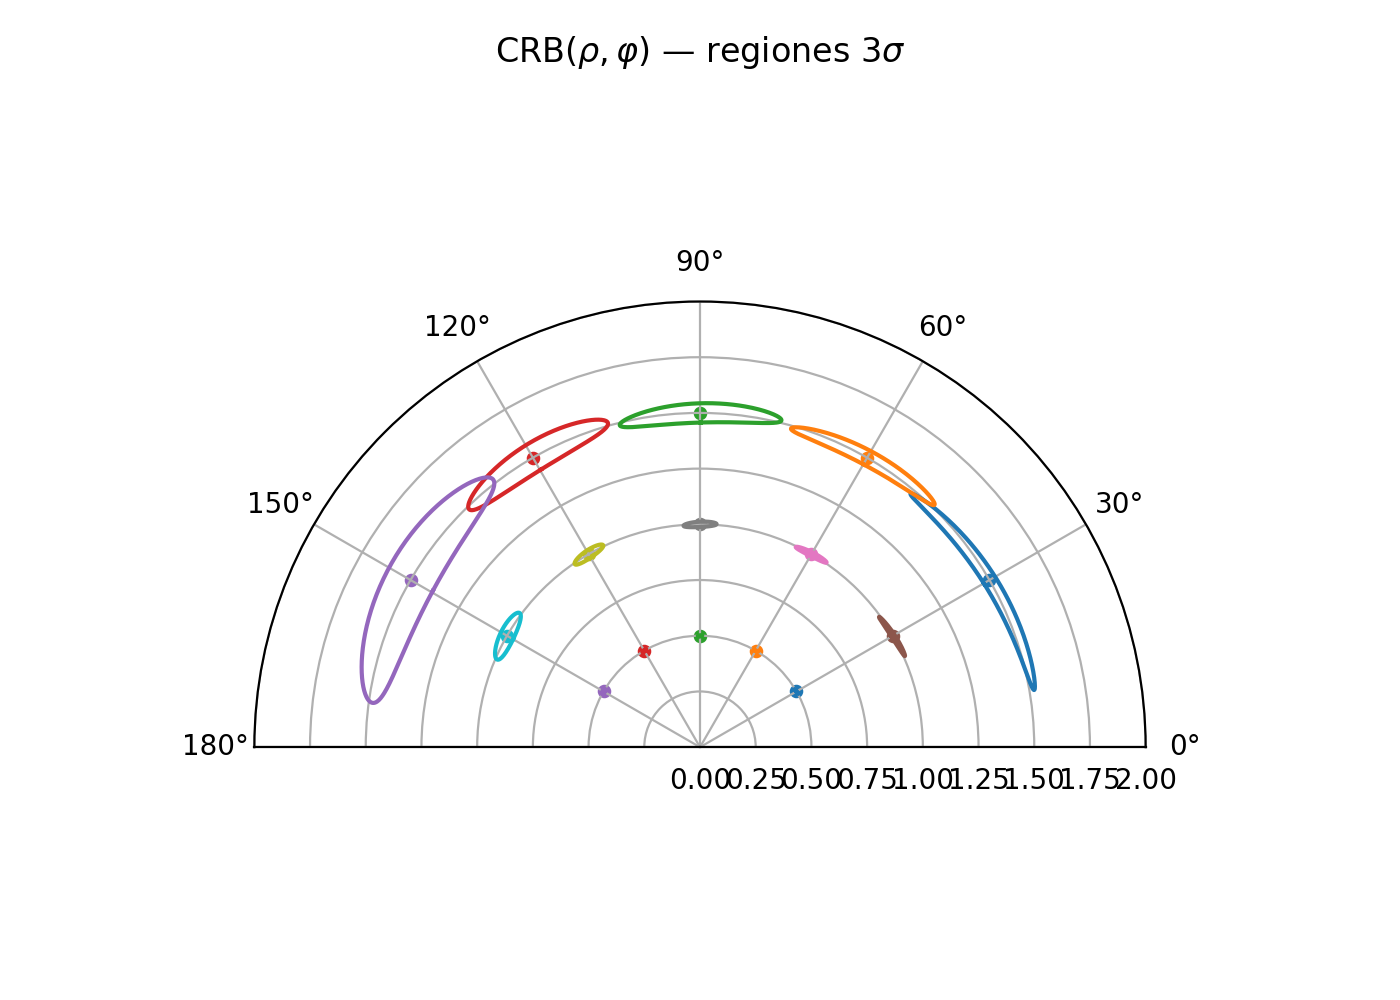
\includegraphics[width=0.92\textwidth]{../plots/crb_standard_regions_fixed_h.png}%
}{%
\textit{(Pendiente: regenerar \texttt{crb\_standard\_regions\_fixed\_h.png}.)}%
}
\caption{CRB$(\rho,\varphi)$: regiones $3\sigma$ ($h$ no se estima). Archivo: \texttt{plots/crb\_standard\_regions\_fixed\_h.png}.}
\label{fig:crb-regions-fixed}
\end{figure}

Regenerar ambas:
\texttt{python regenerate\_crb\_standard\_regions.py}.

%==============================================================================
\section{Qu\'e se usa para generar los plots CRB}
\label{sec:flujo}
%==============================================================================

Esta secci\'on describe \textbf{solo la cadena CRB} (derivadas, Fisher, cota,
elipses). El simulador se trata como una caja negra
\texttt{simulation}$(\rho,\varphi,w,h)\mapsto y$.

\subsection{Piezas que intervienen}
\begin{center}
\small
\begin{tabular}{@{}p{4.6cm}p{9.1cm}@{}}
\toprule
Pieza & Para qu\'e sirve en el CRB \\
\midrule
\texttt{simulation(...)} (notebook) &
Da el histograma esperado $y$ en una pose. No calculamos derivadas aqu\'i. \\
\texttt{forward\_g\_polar} &
Forma $g=y+b$ (vector de todos los bins SPAD$\times$tiempo). \\
\texttt{finite\_difference\_jacobian\_polar} &
Aproxima $\partial g/\partial\psi_m$ por diferencias finitas centrales. \\
\texttt{fisher\_poisson} &
Arma $\matr{I}=\matr{J}^{\mathsf T}\diag(1/g)\,\matr{J}$. \\
\texttt{compute\_crb\_polar} &
Invierte $\matr{I}$, saca $\sigma$ y la elipse $3\sigma$. \\
\texttt{compute\_crb\_grid\_polar} &
Repite lo anterior en la malla de poses. \\
\texttt{plot\_crb\_regions\_polar} &
Dibuja las elipses en ejes polares y guarda el PNG. \\
\texttt{regenerate\_crb\_standard\_regions.py} &
Ejecuta el grid sin Jupyter (modos CRB$(\rho,\varphi,h)$ y CRB$(\rho,\varphi)$). \\
\bottomrule
\end{tabular}
\end{center}

\subsection{Paso 1 --- tasa esperada $g$}
En la pose nominal $\vect{\psi}_0$ (p.\ ej.\ $[\rho_0,\varphi_0,h_0]$):
\[
y_0=\texttt{simulation}(\vect{\psi}_0),\qquad
g_0=\operatorname{vec}(y_0+b).
\]
$b$ es el fondo (\texttt{background\_rate}). $g_0$ incluye bins en sombra
($y\approx 0$). C\'odigo en \texttt{crb\_polar\_functions.py}:
\begin{lstlisting}
# g = y + b  (forward_g_polar)
y_signal, params = simulate_facet_signal_expected(...)  # llama simulation
background = float(background_rate) * np.ones_like(y_signal)
g = y_signal + background
return g, y_signal, params

# desde psi = [rho, phi] o [rho, phi, h]  (forward_g_from_psi)
g, y_signal, params = forward_g_polar(..., height=h, ...)
return np.asarray(g, dtype=float).ravel(), y_signal, params
\end{lstlisting}

\subsection{Paso 2 --- Jacobiano por diferencias finitas}
Para cada par\'ametro $\psi_m\in\{\rho,\varphi\}$ o $\{\rho,\varphi,h\}$:
\begin{equation}
    J_{\cdot m}
    \approx
    \frac{
        g(\vect{\psi}_0+\delta_m\vect{e}_m)
        -
        g(\vect{\psi}_0-\delta_m\vect{e}_m)
    }{2\delta_m}.
\end{equation}
Pasos t\'ipicos: $\delta\rho=0{,}01\,\mathrm{m}$,
$\delta\varphi=0{,}5^\circ$, $\delta h=0{,}01\,\mathrm{m}$.
\begin{lstlisting}
# finite_difference_jacobian_polar  (nucleo)
g0, y0, params0 = forward_g_from_psi(psi0, ...)
J = np.zeros((g0.size, n), dtype=float)
for m in range(n):
    dpsi = np.zeros(n); dpsi[m] = steps[m]
    g_p, _, _ = forward_g_from_psi(psi0 + dpsi, ...)
    g_m, _, _ = forward_g_from_psi(psi0 - dpsi, ...)
    J[:, m] = (g_p - g_m) / (2.0 * steps[m])
return g0, J, y0, params0
\end{lstlisting}

\subsection{Paso 3 --- Fisher y CRB}
\begin{equation}
    \matr{I}
    =
    \matr{J}^{\mathsf T}\diag(1/g_0)\,\matr{J},
    \qquad
    \mathrm{CRB}
    =
    \matr{I}^{+}.
\end{equation}
\begin{lstlisting}
# fisher_poisson
g_safe = np.maximum(g, eps)
I = J.T @ ((1.0 / g_safe)[:, None] * J)

# dentro de compute_crb_polar
g0, J, y0, params0, method = compute_jacobian_polar(...)
I = fisher_poisson(g0, J, eps=fisher_eps)
CRB = np.linalg.pinv(I)
sigma_rho = np.sqrt(CRB[0, 0])
sigma_phi = np.sqrt(CRB[1, 1])
# si 3x3: sigma_height = np.sqrt(CRB[2, 2])
\end{lstlisting}

\subsection{Paso 4 --- elipse $3\sigma$ y plot}
Bloque $2\times 2$ de $(\rho,\varphi)$ (marginal si Fisher es $3\times 3$):
\begin{lstlisting}
# crb_region_in_polar_parameters
Sigma = CRB[np.ix_([0, 1], [0, 1])]
evals, evecs = np.linalg.eigh(Sigma)
t = np.linspace(0, 2*np.pi, n_points)
circle = np.vstack([np.cos(t), np.sin(t)])
axes = k * np.sqrt(np.maximum(evals, 0))
center = np.array([rho0, phi0])
ellipse = center[:, None] + evecs @ np.diag(axes) @ circle
rho_curve, phi_curve = ellipse[0], ellipse[1]

# plot_crb_regions_polar
fig, ax = plt.subplots(subplot_kw={"projection": "polar"})
for result in results:
    ax.plot(result["phi_curve_param"], result["rho_curve_param"])
    ax.scatter([result["phi0"]], [result["rho0"]], s=15)
ax.set_thetamin(0); ax.set_thetamax(180)
fig.savefig(output_path, dpi=dpi)
\end{lstlisting}

\subsection{Dos plots (llamada al grid)}
\begin{lstlisting}
# CRB(rho, phi, h)  ->  plots/crb_standard_regions.png
results_h = compute_crb_grid_polar(
    ..., estimate_height=True,
    finite_difference_steps=[0.01, np.deg2rad(0.5), 0.01],
)
plot_crb_regions_polar(
    results_h, use_physical_region=False, rlim=2.0,
    title="CRB(rho, phi, h) - regiones 3 sigma",
    output_path="plots/crb_standard_regions.png",
)

# CRB(rho, phi)  ->  plots/crb_standard_regions_fixed_h.png
results_fixed = compute_crb_grid_polar(
    ..., estimate_height=False,
    finite_difference_steps=[0.01, np.deg2rad(0.5)],
)
plot_crb_regions_polar(
    results_fixed, use_physical_region=False, rlim=2.0,
    title="CRB(rho, phi) - regiones 3 sigma",
    output_path="plots/crb_standard_regions_fixed_h.png",
)
\end{lstlisting}

\subsection{Orquestaci\'on}
\texttt{compute\_crb\_polar} = pasos 1--4 en una pose.
\texttt{compute\_crb\_grid\_polar} = bucle en
$\rho\in\{0{,}5,1{,}0,1{,}5\}$,
$\varphi\in\{30^\circ,\ldots,150^\circ\}$.
El notebook o
\texttt{regenerate\_crb\_standard\_regions.py}
llaman al grid y guardan el PNG.

\end{document}
